\chapter{Benchmarking AO-DF-SOS-ADC(2)}

The theoretical groundwork for AO-DF-SOS-ADC(2) was laid out in detail in the previous chapters. In this chapter, the performance of the method and its components will be anylyzed \emph{in silico}. First, a brief overview is given on the computational details, as well as on the types of molecular systems that are taken into consideration. Then, the scaling, memory foot-print and accuracy of the J,K and Z kernels is analyzed for different metrics in the context of Hartree-Fock and MP2. It serves also also as a mean to get a first grip on the performance of quasi-robust density fitting. Finally, the AO-DF-SOS-ADC(2) method is anaylzed in the last part.  

\section{Computational Details}

All results presented in this chapter were obtained using MEGALOchem, an open-source quantum chemistry package which specializes in algorithms expliting sparsity. For more details, the reader is referred to the user's guide and the developer's guide in chapter ... and ... 

All calculations were performed on ...

\section{Molecular Test Systems}

Virtually all works that present some form of low-scaling electronic structure methods use linear alkanes (LA) as their test systems. Linear molecular system represent a best case scenario where the overlap between basis functions decays very rapidly as function of distance. The low scaling regime can generally be reached quite quickly, which is great for getting a first impression on the performance on the methods. Unfortunately, linear systems like alkanes are chemically uninteresting. For this reason, the present benchmarking also looks at the worst case scenario of spherically shaped molecular system, in this case solvated formamide (FW) with differently sized solvation shells. For systems such as these, electron correlation descreases very slowly as function of increasing system size $N$. The LA and FW systems are used to analyze the performance of the kernels.

Another type of system is introduced for AO-DF-SOS-ADC(2): linear carboxlyic acids (LC). The domain for the lowest lying domain is entirely located on the functional group COOH ($\pi\rightarrow\pi*$, Figure ...). This class of molecules represents the absolute best case scenario for local excitation methods: fast decay of correlation effects as a function of distance due to its linearity, and a very localized excitation domain. 

This other form of locality is also the reason why the FW systems were chosen instead of simple water clusters: while correlation effects decay slowly, the excitation domain for the lowest reason is localized on the formamide molecule (ref). These systems represent an interesting mix between different types of locality and non-locality and give insight on how local excited state methods handle these fringe cases. 

Four different sizes are chosen for each system type in a manner that they have a comparable number of basis functions to allow a better comparison.

Only basis sets with double-zeta quality were considered (cc-pVDZ, def2-SVP, aug-cc-pVDZ, def2-SVPD) due to time and resource constraints. It is expected that the methods still suffer from an $\ccpx{4}$ scaling as a function of basis set size. The number of basis functions for the different

\begin{figure}
     \centering
     \begin{subfigure}{0.4\textwidth}
         \centering
         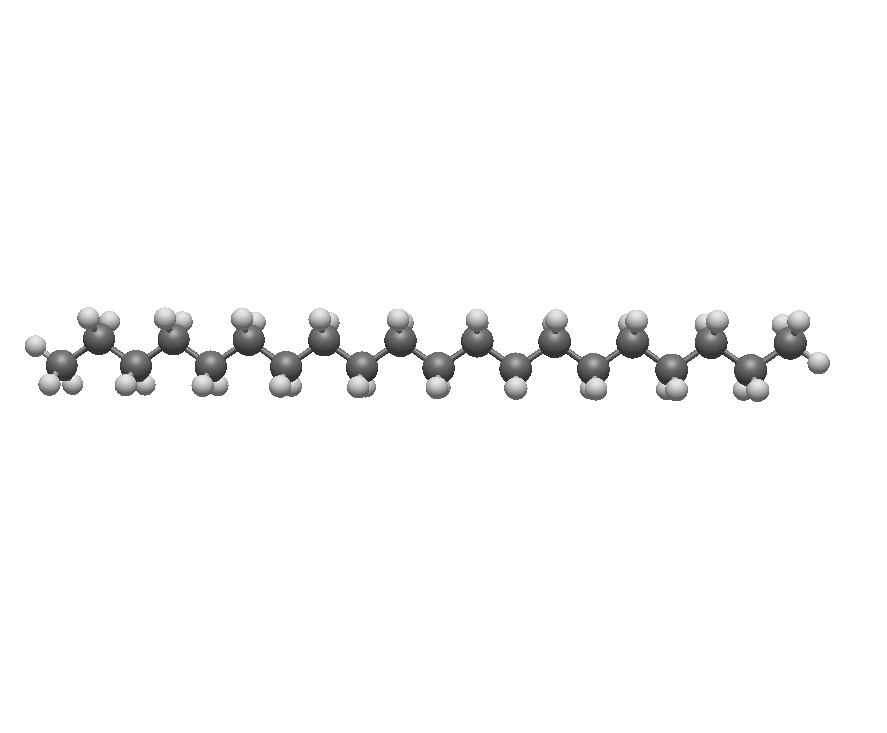
\includegraphics[width=\textwidth]{Pics/alkan.png}
         \caption{$y=x$}
         \label{fig:y equals x}
     \end{subfigure}
	\begin{subfigure}{0.5\textwidth}
         \centering
         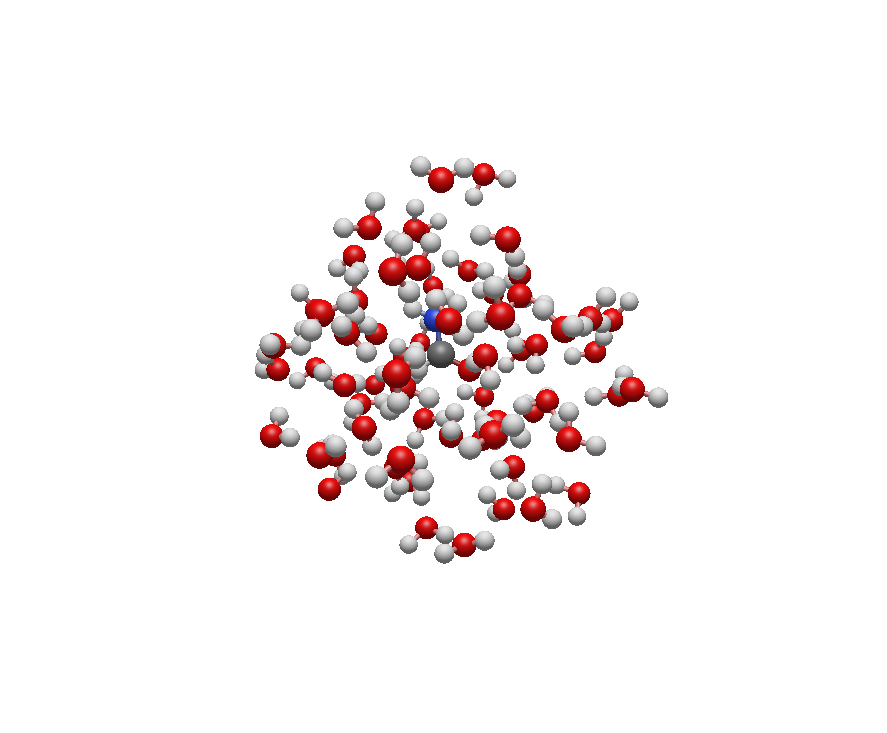
\includegraphics[width=\textwidth]{Pics/FW63.png}
         \caption{$y=5/x$}
         \label{fig:five over x}
     \end{subfigure}
     \hfill
     \begin{subfigure}{0.4\textwidth}
         \centering
         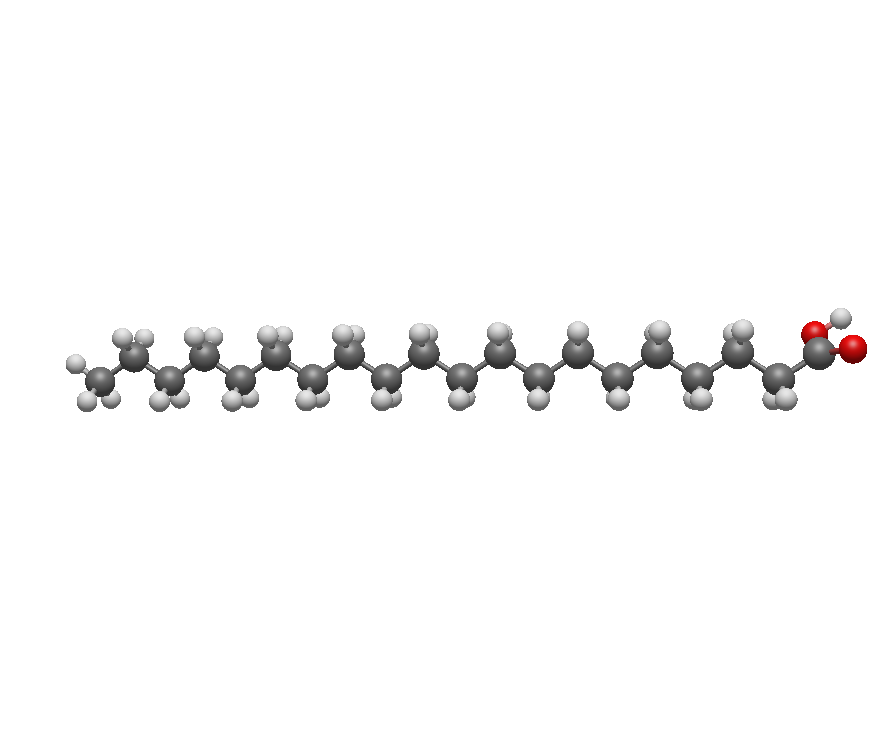
\includegraphics[width=\textwidth]{Pics/acid.png}
         \caption{$y=3sinx$}
         \label{fig:three sin x}
     \end{subfigure}
     \hfill
     
        \caption{Three simple graphs}
        \label{fig:three graphs}
\end{figure}

\begin{table}
\centering
\begin{tabular}{cc|cc|cc}
\hline
\multicolumn{2}{c}{LA} & \multicolumn{2}{c}{FW} & \multicolumn{2}{c}{LC}\\ \hline
Molecule & $N_{AO}$ & Molecule & $N_{AO}$ & Molecule & $N_{AO}$ \\ \hline
H$_{42}$C$_{20}$ & 490 & H$_{33}$CNO$_{16}$ & 417 & H$_{40}$C$_{20}$O$_2$ & 508 \\
H$_{82}$C$_{40}$ & 970 & H$_{63}$CNO$_{31}$ & 777 & H$_{80}$C$_{40}$O$_2$ & 988 \\
H$_{162}$C$_{80}$ & 1930 & H$_{129}$CNO$_{64}$ & 1569 & H$_{160}$C$_{80}$O$_2$ & 1948 \\
H$_{322}$C$_{160}$ & 3850 & H$_{291}$CNO$_{145}$ & 3513 & H$_{320}$C$_{160}$O$_2$ & 3868  
\end{tabular}
\label{MOLBASIS1}
\caption{Molecular formula for the considered systems and the number of basis functions when using cc-pVDZ}
\end{table}

\section{Ground-State Prerequisites}

\subsection{Hartree-Fock}

% density/scaling of B
\begin{figure*}
\begin{minipage}{0.5\textwidth}
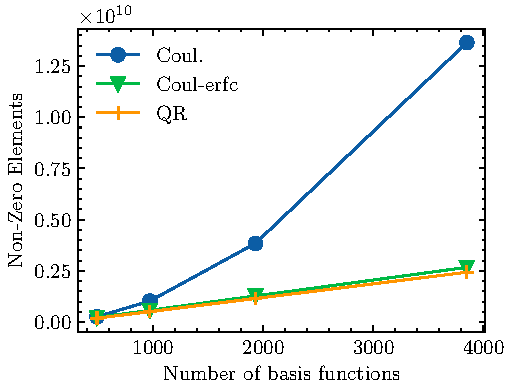
\includegraphics[width=\textwidth]{../articles/art1/eri_nze_alkan}
\captionof{figure}[This Figure]{Figure}
\end{minipage}
\hspace{0.05\textwidth}
\begin{minipage}{0.3\textwidth}
\begin{tabular}{rrrr}
\hline
N$_{AO}$ & Coul. & Coul-erfc & QR \\ \hline
490 & --- & --- & --- \\ 
970 & 2.01 & 1.37 & 1.45 \\ 
1930 & 1.92 & 1.16 & 1.18 \\ 
3850 & 1.83 & 1.07 & 1.08 \\ \hline
\end{tabular}
\captionof{table}[This Table]{Table}
\end{minipage}
\end{figure*}
%
\begin{figure*}
\begin{minipage}{0.5\textwidth}
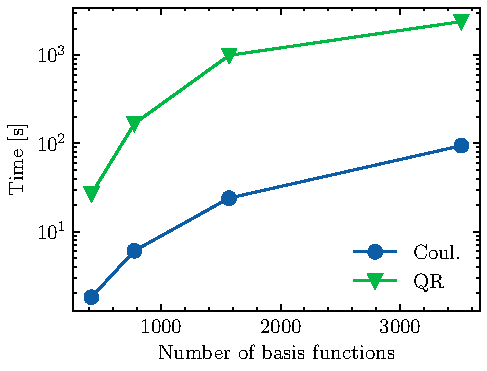
\includegraphics[width=\textwidth]{../articles/art1/qrtime_alkan}
\captionof{figure}[This Figure]{Figure}
\end{minipage}
\hspace{0.05\textwidth}
\begin{minipage}{0.3\textwidth}
\begin{tabular}{rrr}
\hline
N$_{AO}$ & Coul. & QR \\ \hline
490 & --- & --- \\ 
970 & 1.94 & 2.95 \\ 
1930 & 1.96 & 2.53 \\ 
3850 & 1.70 & 1.09 \\ \hline
\end{tabular}
\captionof{table}[This Table]{Table}
\end{minipage}
\end{figure*}
%
\begin{figure*}
\begin{minipage}{0.5\textwidth}
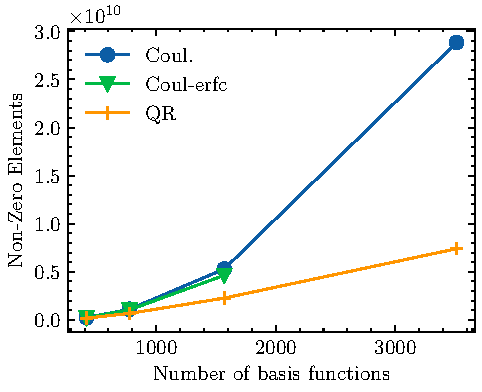
\includegraphics[width=\textwidth]{../articles/art1/eri_nze_fw}
\captionof{figure}[This Figure]{Figure}
\end{minipage}
\hspace{0.05\textwidth}
\begin{minipage}{0.3\textwidth}
\begin{tabular}{rrrr}
\hline
N$_{AO}$ & Coul. & Coul-erfc & QR \\ \hline
417 & --- & --- & --- \\ 
777 & 2.50 & 2.45 & 2.15 \\ 
1569 & 2.23 & 2.11 & 1.73 \\ 
3513 & 2.10 & --- & 1.47 \\ \hline
\end{tabular}
\captionof{table}[This Table]{Table}
\end{minipage}
\end{figure*}
%
\begin{figure*}
\begin{minipage}{0.5\textwidth}
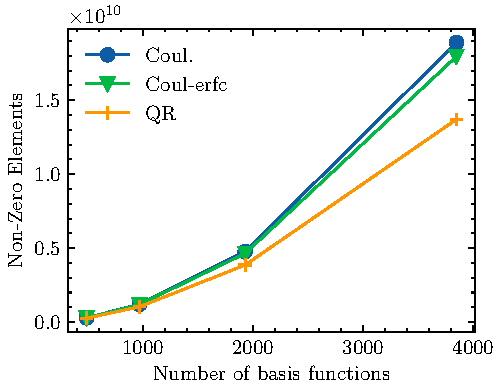
\includegraphics[width=\textwidth]{../articles/art1/cfit_nze_alkan}
\captionof{figure}[This Figure]{Figure}
\end{minipage}
\hspace{0.05\textwidth}
\begin{minipage}{0.3\textwidth}
\begin{tabular}{rrrr}
\hline
N$_{AO}$ & Coul. & Coul-erfc & QR \\ \hline
490 & --- & --- & --- \\ 
970 & 2.07 & 2.06 & 2.01 \\ 
1930 & 2.01 & 1.98 & 1.92 \\ 
3850 & 1.99 & 1.96 & 1.84 \\ \hline
\end{tabular}
\captionof{table}[This Table]{Table}
\end{minipage}
\end{figure*}
%
\begin{figure*}
\begin{minipage}{0.5\textwidth}
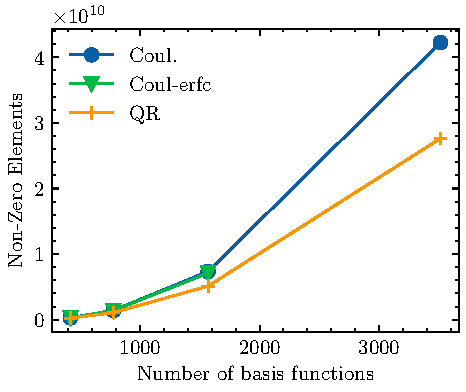
\includegraphics[width=\textwidth]{../articles/art1/cfit_nze_fw}
\captionof{figure}[This Figure]{Figure}
\end{minipage}
\hspace{0.05\textwidth}
\begin{minipage}{0.3\textwidth}
\begin{tabular}{rrrr}
\hline
N$_{AO}$ & Coul. & Coul-erfc & QR \\ \hline
417 & --- & --- & --- \\ 
777 & 2.27 & 2.26 & 2.20 \\ 
1569 & 1.96 & 1.94 & 1.88 \\ 
3513 & 1.71 & 1.68 & 1.57 \\ \hline
\end{tabular}
\captionof{table}[This Table]{Table}
\end{minipage}
\end{figure*}
%
\begin{figure*}
\begin{minipage}{0.5\textwidth}
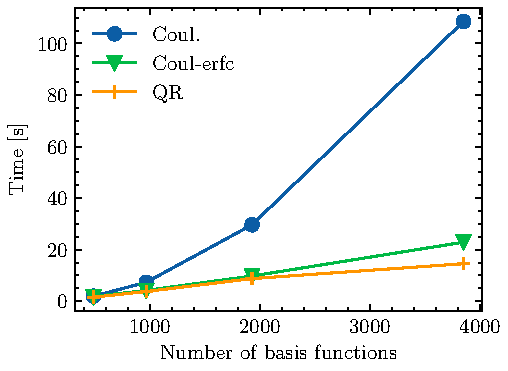
\includegraphics[width=\textwidth]{../articles/art1/hfJ_alkan}
\captionof{figure}[This Figure]{Figure}
\end{minipage}
\hspace{0.05\textwidth}
\begin{minipage}{0.3\textwidth}
\begin{tabular}{rrrr}
\hline
N$_{AO}$ & Coul. & Coul-erfc & QR \\ \hline
490 & --- & --- & --- \\ 
970 & 1.93 & 1.23 & 1.29 \\ 
1930 & 2.03 & 1.23 & 1.23 \\ 
3850 & 1.88 & 1.23 & 0.73 \\ \hline
\end{tabular}
\captionof{table}[This Table]{Table}
\end{minipage}
\end{figure*}
%
\begin{figure*}
\begin{minipage}{0.5\textwidth}
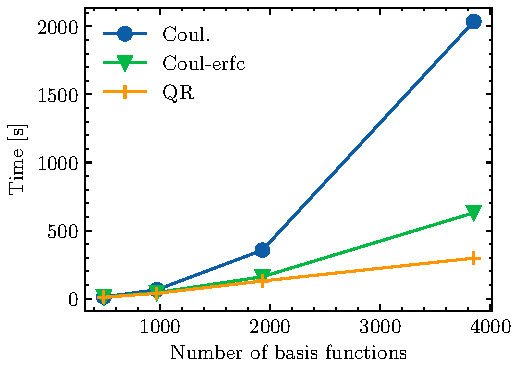
\includegraphics[width=\textwidth]{../articles/art1/hfK1_alkan}
\captionof{figure}[This Figure]{Figure}
\end{minipage}
\hspace{0.05\textwidth}
\begin{minipage}{0.3\textwidth}
\begin{tabular}{rrrr}
\hline
N$_{AO}$ & Coul. & Coul-erfc & QR \\ \hline
490 & --- & --- & --- \\ 
970 & 2.43 & 1.97 & 1.96 \\ 
1930 & 2.49 & 1.89 & 1.78 \\ 
3850 & 2.53 & 1.98 & 1.21 \\ \hline
\end{tabular}
\captionof{table}[This Table]{Table}
\end{minipage}
\end{figure*}
%
\begin{figure*}
\begin{minipage}{0.5\textwidth}
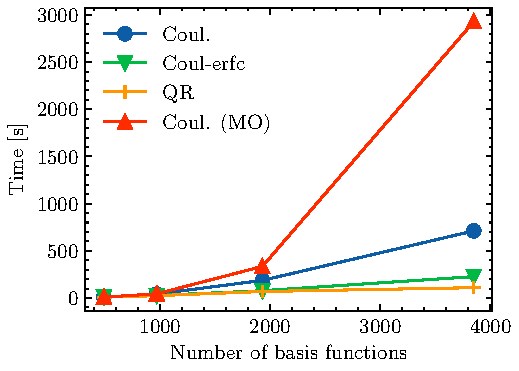
\includegraphics[width=\textwidth]{../articles/art1/hfK2_alkan}
\captionof{figure}[This Figure]{Figure}
\end{minipage}
\hspace{0.05\textwidth}
\begin{minipage}{0.3\textwidth}
\begin{tabular}{rrrrr}
\hline
N$_{AO}$ & Coul. & Coul-erfc & QR & Coul. (MO) \\ \hline
490 & --- & --- & --- & --- \\ 
970 & 1.58 & 1.58 & 1.60 & 2.34 \\ 
1930 & 1.57 & 1.57 & 1.50 & 2.96 \\ 
3850 & 1.56 & 1.56 & 0.67 & 3.14 \\ \hline
\end{tabular}
\captionof{table}[This Table]{Table}
\end{minipage}
\end{figure*}

\begin{table}
\begin{tabular}{r|rrr|rrr|rrrr}
\hline
 & \multicolumn{3}{c}{J} & \multicolumn{3}{c}{K (STEP 1)} &   \multicolumn{4}{c}{K (STEP 2)} \\ \hline
N$_{AO}$ & Coul. & Erfc & QR & Coul. & Erfc & QR & Coul. & Erfc & QR & Coul. (MO) \\ \hline
417 & --- & --- & --- & --- & --- & --- & --- & --- & --- & --- \\ 
777 & 2.18 & 2.20 & 1.88 & 2.77 & 2.77 & 2.51 & 2.55 & 2.55 & 2.33 & 2.33 \\ 
1569 & 2.32 & 1.71 & 1.28 & 2.77 & 2.18 & 1.85 & 2.82 & 2.13 & 1.67 & 2.86 \\ 
3513 & 2.08 & --- & 1.94 & 2.79 & --- & 2.74 & 2.59 & --- & 2.65 & 3.13 \\ \hline
\end{tabular}
\caption{Here}
\label{}
\end{table}

\subsection{MP2}

\begin{figure*}
\begin{minipage}{0.5\textwidth}
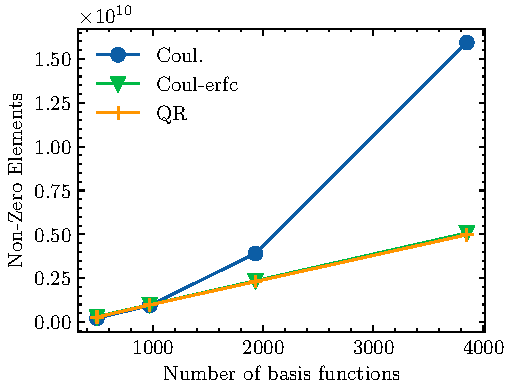
\includegraphics[width=\textwidth]{../articles/art1/ftmp2_nze_alkan}
\captionof{figure}[This Figure]{Figure}
\end{minipage}
\hspace{0.05\textwidth}
\begin{minipage}{0.3\textwidth}
\begin{tabular}{rrrr}
\hline
N$_{AO}$ & Coul. & Coul-erfc & QR \\ \hline
490 & --- & --- 	& --- \\ 
970	& 2.14 & 2.13 & 2.12 \\
1930	 & 2.06 & 2.06 & 2.06 \\
3850	 & 2.03 & 2.03 & 2.03 \\
 \hline
\end{tabular}
\captionof{table}[This Table]{REDO THIS!!!!}
\end{minipage}
\end{figure*}

\begin{figure*}
\begin{minipage}{0.5\textwidth}
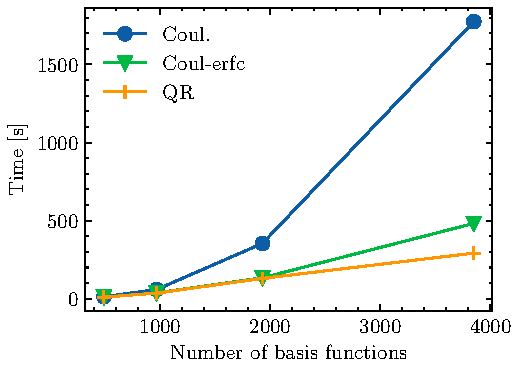
\includegraphics[width=\textwidth]{../articles/art1/mp2_alkan}
\captionof{figure}[This Figure]{Figure}
\end{minipage}
\hspace{0.05\textwidth}
\begin{minipage}{0.3\textwidth}
\begin{tabular}{rrrr}
\hline
N$_{AO}$ & Coul. & Coul-erfc & QR \\ \hline
490 & --- & --- 	& --- \\ 
970	& 2.45 & 1.96 & 2.09 \\
1930	 & 2.55 & 1.82 & 1.83 \\
3850	 & 2.00 & 1.59 & 1.00 \\
 \hline
\end{tabular}
\captionof{table}[This Table]{REDO THIS!!!!}
\end{minipage}
\end{figure*}

\begin{table}
\begin{tabular}{rrrr}
N$_{AO}$ & Coul. & Coul-erfc & QR \\ 
490 & --- & --- & --- \\ 
970 & 2.51 & 1.88 & 1.88 \\ 
1930 & 2.59 & 3.18 & 2.36 \\ 
3850 & 3.26 & 3.18 & --- \\ 
\end{tabular}
\caption{Here}
\label{}
\end{table}

\section{Excited-State}